\documentclass{standalone}
\usepackage{tikz}
\begin{document}
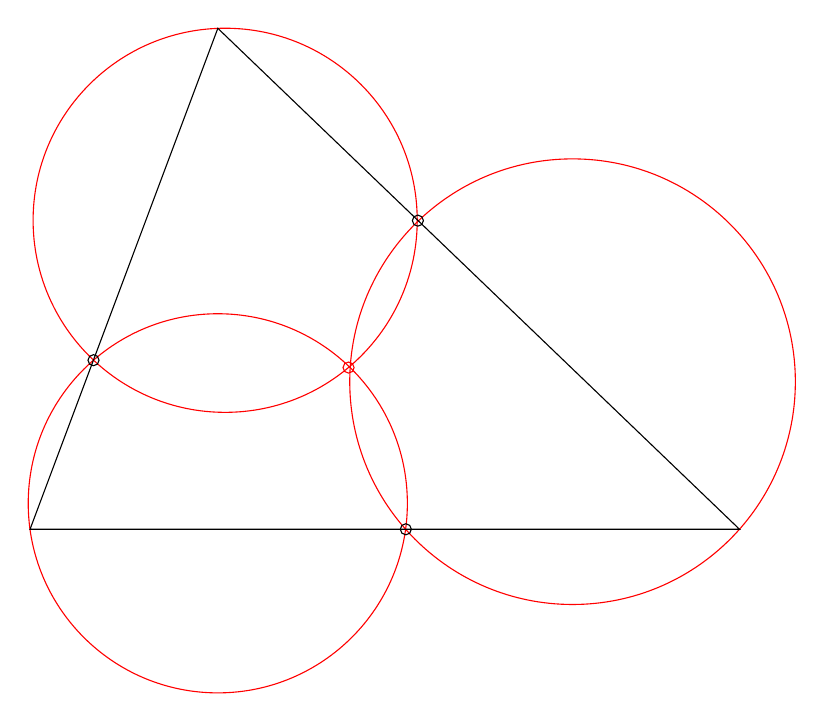
\begin{tikzpicture}[x=1pt,y=1pt]
\draw[red] (86.89,-91.03) circle (69.40);
\draw[red] (212.42,-149.35) circle (80.51);
\draw[red] (84.23,-193.30) circle (68.50);
\draw (272.75,-202.68) -- (16.38,-202.68) -- (84.24,-21.66) -- cycle;
\draw (39.32,-141.59) circle (2.00);
\draw[red] (131.48,-144.25) circle (2.00);
\draw (152.17,-202.68) circle (2.00);
\draw (156.53,-91.15) circle (2.00);
\end{tikzpicture}
\end{document}
